
\chapter{矩阵}
\label{chap:matrix}

通俗地讲,矩阵就是$n\times m$个东西排列成一个$n\times m$的矩形阵列。在数学上,阵列里的东西通常是各种各样的“数”,实数、复数、函数等。

\section{行列式}
\label{sec:determinant}

行列式(Determinant)是针对$n\times n$的方阵的概念,方阵$A$的行列式通常用$\left| A\right|$或者$\det(A)$表示。二阶方阵的行列式为
\begin{align*}
  \begin{vmatrix}
    a_{11} & a_{12}\\
    a_{21} & a_{22}
  \end{vmatrix}
             \equiv a_{11}a_{22} - a_{12}a_{21}
\end{align*}

三阶方阵的行列式为
\begin{align*}
  \begin{vmatrix}
    a_{11} & a_{12} & a_{13}\\
    a_{21} & a_{22} & a_{23}\\
    a_{31} & a_{32} & a_{33}
  \end{vmatrix}\equiv
   a_{11}\begin{vmatrix} a_{22} & a_{23}\\ a_{32} & a_{33} \end{vmatrix}
  -a_{21}\begin{vmatrix} a_{12} & a_{13}\\ a_{32} & a_{33} \end{vmatrix}
  +a_{31}\begin{vmatrix} a_{12} & a_{13}\\ a_{22} & a_{23} \end{vmatrix}
\end{align*}

同样可以递归地用$n$阶方阵的行列式定义$n+1$阶方阵的行列式。若要深入系统地学习了解高阶矩阵的,请移步参考高等代数、矩阵分析等相关教材。

\begin{example}[萨吕法则,Sarrus' Rule,Sarrus' Scheme]
  将$3\times 3$的矩阵
  \begin{align*}
    M =
    \begin{pmatrix}
      a_{11} & a_{12} & a_{13}\\
      a_{21} & a_{22} & a_{23}\\
      a_{31} & a_{32} & a_{33}
    \end{pmatrix}
  \end{align*}
  按图~\ref{fig:Sarrus'-rule}扩充为$3\times 5$的矩阵并沿对角线作出辅助线:
  \begin{figure}[htbp]
    \centering
    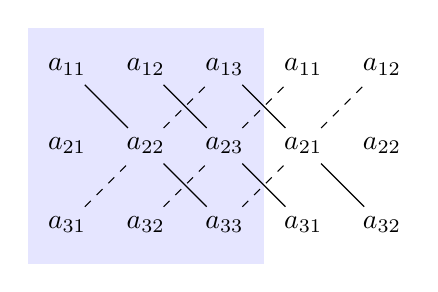
\begin{tikzpicture}[scale=1]
      \fill[color=blue!10](-.5,.5)rectangle(2.5,-2.5);
      \foreach \x/\y/\v/\i in{0/0/11/11, 1/0/12/12, 2/0/13/13, 3/0/11/e11, 4/0/12/e12,
                              0/1/21/21, 1/1/22/22, 2/1/23/23, 3/1/21/e21, 4/1/22/e22,
                              0/2/31/31, 1/2/32/32, 2/2/33/33, 3/2/31/e31, 4/2/32/e32}{
        \node(N\i) at (\x, -\y){$a_{\v}$};
      }
      \foreach \a/\b/\c in {11/22/33,12/23/e31,13/e21/e32}{
        \draw(N\a)--(N\b) (N\b)--(N\c);
      }
      \foreach \a/\b/\c in {31/22/13,32/23/e11,33/e21/e12}{
        \draw[dashed](N\a)--(N\b) (N\b)--(N\c);
      }
    \end{tikzpicture}
    \caption{萨吕法则}
    \label{fig:Sarrus'-rule}
  \end{figure}
  
  则按实线三数乘积取正,虚线三数乘积取负,然后求和,可得$\det(M)$为
  \begin{align*}
    \det(M) ={}& +a_{11}a_{22}a_{33} + a_{12}a_{23}a_{31} + a_{13}a_{21}a_{32}\\
               & -a_{31}a_{22}a_{13} + a_{32}a_{23}a_{11} - a_{33}a_{21}a_{12}
  \end{align*}
\end{example}

\begin{theorem}[三角形面积的行列式公式]
  记平面直角坐标系下三角形的3个顶点的坐标分别为$(x_1, y_1)$,$(x_2,y_2)$和$(x_3,y_3)$,则三角形的面积为
  \begin{align*}
    S =\left| \det
    \begin{pmatrix}
      x_1 & y_1 & 1\\
      x_2 & y_2 & 1\\
      x_3 & y_3 & 1
    \end{pmatrix}\right|
  \end{align*}
\end{theorem}


\section{向量}
\label{sec:vector}

通常$1\times n$的敌阵称为行向量,$n\times 1$的矩阵称为列向量,行向量与列向量都是向量,通常在上下文能确定是行向量还是列向量时,行列两字会省略。

\subsection{点积}
\label{sec:dot-product-of-vector}
\begin{definition}
  两个向量对应分量的积之和称为点积(dot product),也称为数量积,通常记为$\vec a\cdot\vec b$或者$(\vec a,\vec b)$,或者$\langle\vec a,\vec b\rangle$,即
  \begin{align*}
    \vec{a}\cdot \vec b\equiv\sum_i a_ib_i
  \end{align*}
\end{definition}

显然,点积是满足交换律与分配律的,即
\begin{align*}
  \vec a\cdot \vec b={}&\vec b\cdot \vec a\\
  (\vec a + \vec b)\cdot \vec c ={}& \vec a\cdot \vec c + \vec b\cdot \vec c
\end{align*}

\begin{theorem}
  三维欧氏空间中任意两向量,有
  \begin{align*}
    \vec{a}\cdot \vec b=\left|\vec a\right| \cdot \left|\vec b\right| \cos\theta
  \end{align*}
  其中$\theta$是两向量之间的夹角,从而两向量之间夹角的余弦为
  \begin{align*}
    \cos\theta = \frac{\vec a\cdot \vec b}{\left|\vec a\right| \cdot \left|\vec b\right|}
  \end{align*}
\end{theorem}
\begin{proof}[提示]
  利用余弦定理。
  \begin{center}
    \begin{tikzpicture}[scale=1.0]
      \coordinate(O)at(0,0);
      \coordinate(A)at(3,0);
      \coordinate(B)at(2,2);
      \draw pic["$\theta$",<->,draw=orange,angle eccentricity=1.6,angle radius=.6cm]{angle=A--O--B};
      \draw[->](O)--(A)node[midway,below]{$\vec a$};
      \draw[->](O)--(B)node[midway,sloped,above]{$\vec b$};
      \draw[->](B)--(A)node[midway,sloped,above]{$\vec a - \vec b$};
    \end{tikzpicture}
  \end{center}
  由余弦定理,有
  \begin{align*}
    (\vec a-\vec b)\cdot(\vec a-\vec b) = \vec a\cdot \vec a + \vec b\cdot\vec b
    - 2\left|\vec a\right|\cdot\left|\vec b\right|\cos\theta
  \end{align*}
  展开可得。
\end{proof}

\begin{example}[平面向量的旋转]
  记$\vec a$是平面上二维向量,其在直角坐标系下的两分量为$a_x$与$a_y$,即
  \begin{align*}
    \vec a\equiv
    \begin{pmatrix}
      a_x\\ a_y
    \end{pmatrix}
  \end{align*}
  现将向量沿坐标原点逆时针旋转$\theta$度,记旋转后得到的向量为$\vec a'$。若分别用复数$z$与$z'$表示向量$\vec a$和$\vec a'$,则有
  \begin{align*}
    z' ={}& z\cdot e^{i\theta} = (\cos\theta + i\sin\theta)\cdot (a_x + i a_y)\\
       ={}& \cos\theta a_x - \sin\theta a_y + i(\sin\theta a_x + \cos\theta a_y)\\
       ={}& (\cos\theta,\ -\sin\theta)\begin{pmatrix}a_x\\a_y\end{pmatrix} + i
            (\sin\theta,\  \cos\theta)\begin{pmatrix}a_x\\a_y\end{pmatrix}
  \end{align*}
  写成矩阵的形式,就有
  \begin{align*}
    \begin{pmatrix}
      a_x'\\ a_y'
    \end{pmatrix}=
    \begin{pmatrix}
      \cos\theta & -\sin\theta\\
      \sin\theta & \phantom{-}\cos\theta
    \end{pmatrix}
    \begin{pmatrix}
      a_x\\ a_y
    \end{pmatrix}
  \end{align*}
  上式中的矩阵称为旋转矩阵(Rotate Matrix)。
\end{example}

\begin{example}[垂直向量]
  逆时针旋转$90^\circ$,即旋转矩阵中$\theta$取为$\pi/2$。记旋转后的向量为$\vec a^\perp$,则有
  \begin{align*}
    \vec a^\perp = 
    \begin{pmatrix}
      a_x^\perp\\ a_y^\perp
    \end{pmatrix}=
    \begin{pmatrix}
      0 & -1\\
      1 & \phantom{-}0
    \end{pmatrix}
    \begin{pmatrix}
      a_x\\ a_y
    \end{pmatrix}=
    \begin{pmatrix}
      -a_y\\ a_x
    \end{pmatrix}
  \end{align*}
  若是顺时针旋转$90^\circ$,则可以得到另一个垂直向量$(a_y,\ -a_x)^T$,其中$^T$表示转置。
\end{example}

\begin{definition}[Perp Dot Product]
  
\end{definition}


\subsection{叉积}
\label{sec:cross-product-of-vector}
\begin{definition}[叉积,外积,法向量,Cross Product]
  三维欧氏空间中的向量的叉积按下式定义:
  \begin{align*}
    \vec{a}\times\vec{b}\equiv
    \begin{vmatrix}
      \ihat  & \jhat  & \khat\\
      a_1    & a_2    & a_3\\
      b_1    & b_2    & b_3
    \end{vmatrix}
  \end{align*}
  其中$\ihat, \jhat, \khat$是三维欧氏空间中正交坐标下的三个单位正交向量。
\end{definition}

\begin{lemma}[bac--cab Rule\footnote{有个简便的记忆方法:发音为BACK--CAB,意为“后面的出租车”。}]
  $\forall \vec a,\vec b,\vec c\in\mathbb{R}^3$,有
  \begin{align*}
    \vec a\times(\vec b\times \vec c)=\vec b(\vec a,\vec c) - \vec c(\vec a,\vec b)
  \end{align*}
\end{lemma}
\begin{proof}
  最直观的证明是直接展开,对比三个分量。这里不再加以描述。

  另一种方法,是待定系数法。不妨设$\vec b\not\parallel\vec c$,否则显然两边都为零向量。由
  \begin{align*}
    \vec b\times\vec c\perp \vec b,\quad \vec b\times\vec c\perp \vec c,\quad
    \vec a\times(\vec b\times\vec c)\perp \vec b\times \vec c
  \end{align*}
  可知$\vec a\times(\vec b\times\vec c)$必在$\vec b$和$\vec c$张成的空间(在这里是一个平面)里\footnote{因为垂直于向量$\vec b\times\vec c$的平面就是$\vec b$和$\vec c$张成的平面。\color{red}补充一下张成空间的概念?},从而$\exists s,t\in\mathbb{R}$,使得
  \begin{align*}
    \vec a\times(\vec b\times\vec c) = s\vec b +t\vec c
  \end{align*}
  两边与$\vec a$作点积,则有
  \begin{align*}
    s(\vec a,\vec b)+t(\vec a,\vec c)=(\vec a, \vec a\times(\vec b\times\vec c))=0
  \end{align*}
  显然
  \begin{align*}
    s=(\vec a,\vec c),\quad
    t=-(\vec a,\vec b)
  \end{align*}
  是上式的其中一组解。{\color{red}但不一定是原待定系数方程的解。需要换一个思路。}

  考虑满足右手法则的单位正交基
  \begin{align*}
    \ihat \equiv \frac{\vec b}{\left|\vec b\right|},\quad
    \jhat \equiv \frac{\vec b^\perp}{\left|\vec b^\perp\right|},\quad
    \khat \equiv \frac{\vec b\times \vec c}{\left|\vec b\times\vec c\right|}
  \end{align*}
  其中$\vec b^\perp$是$\vec b$和$\vec c$张成的平面内$\vec b$向$\vec c$方向旋转$90^\circ$而成的向量。对$\vec a,\vec b,\vec c$按此正交基作正交分解,记分解结果为
  \begin{align*}
    \vec a=(a_1, a_2, a_3)\begin{pmatrix}\ihat\\ \jhat\\ \khat\end{pmatrix}, \quad
    \vec b=(b_1,   0,   0)\begin{pmatrix}\ihat\\ \jhat\\ \khat\end{pmatrix}, \quad
    \vec c=(c_1, c_2,   0)\begin{pmatrix}\ihat\\ \jhat\\ \khat\end{pmatrix}
  \end{align*}
  其中有不少的零,计算可大大简化。代入左边,有
  \begin{align*}
    \vec a\times(\vec b\times\vec c) ={}& (a_1\ihat + a_2\jhat)\times(b_1\ihat \times c_2\jhat)\\
    ={}& (a_1\ihat + a_2\jhat)\times(bc_2\khat) = a_2bc_2\ihat - a_1bc_2\jhat
  \end{align*}
  同样的,考虑右手边则有
  \begin{align*}
    \vec b(\vec a,\vec c) - \vec c(\vec a,\vec b) = (\underline{a_1c_1} + a_2c_2) b_1\ihat  - (a_1b_1)(\underline{c_1\ihat} + c_2\jhat)
    =a_2b_1c_2\ihat - a_1b_1c_2\jhat
  \end{align*}
  从而左右相等。\footnote{这里应用到了点积、叉积是坐标系变换下的不变量,需要补充一下。}
  % 将$\vec c$作按$\vec b$和$\vec b^\perp$两个方向作正交分解,记为
  % \begin{align*}
  %   \vec c={\vec c}_b + {\vec c}_\perp
  % \end{align*}
  % 其中$\vec c_b \parallel \vec b$,$\vec c_\perp \perp \vec b$。同样对$\vec a$作按$\vec b\times \vec c$方向,与$\vec b$和$\vec c$张成的平面这两个方向作正交分解,记其在$\vec b$和$\vec c$张成的平面内的分量为$\vec a_{bc}$,则  
  % \begin{align*}
  %   \vec a\times(\vec b\times \vec c) = \vec a_{bc}\times(\vec b\times \vec c_\perp) \\
  %   s
  % \end{align*}
\end{proof}

\begin{theorem}
  记$\vec p\equiv\vec a\times \vec b$,则$\vec a$,$\vec b$和$\vec p$满足右手法则,且$\vec p$同时垂直于$\vec a$和$\vec b$,且外积$\vec p$的模为$\left|\vec a\right|\cdot\left|\vec b\right|\sin\theta$,其中$\theta$是$\vec a$与$\vec b$的夹角。即
  \begin{gather*}
    (\vec a\times \vec b)\cdot \vec a = (\vec a\times \vec b)\cdot \vec b = 0\\
    \left| \vec a\times \vec b\right| = \left| \vec a\right| \cdot \left| \vec b\right| \sin\theta
  \end{gather*}
\end{theorem}


\begin{example}[垂足坐标]
  $\mathbb{R}^3$不共线的三点$a$,$b$和$c$,求点$c$到过点$a$和$b$的直线的垂足的坐标。
\end{example}
\begin{proof}[提示]
  记各点对应在的向量为$\vec a$,$\vec b$和$\vec c$。则过点$a$和$b$的直线上的任一点$u$对应的向量$\vec u$都可以写为
  \begin{align*}
    \vec u=\vec a + s\cdot(\vec b-\vec a)
  \end{align*}
  其中$s\in\mathbb{R}$,表示该点与$a$的有向距离与$a$、$b$两点间距离的比值,与点$b$同侧为正,异侧为负。由此,要确定$c$在$\overline{ab}$上的投影的坐标,只要确定其投影的长度即可。由点积,可知其投影长度$L_{proj,c}$为
  \begin{alignat*}{3}
    &&L_{proj,c} ={}& (\vec c-\vec a)\cdot \frac{\vec b - \vec a}{\left| \vec b - \vec a \right|}\\
    \implies&& s ={}& \frac{L_{proj,c}}{\left| \vec b - \vec a \right|} =
    \frac{(\vec c-\vec a)\cdot(\vec b - \vec a)}{\left| \vec b - \vec a \right|^2}
  \end{alignat*}
  若记$\vec w$为$\vec b-\vec a$方向的单位向量,即
  \begin{align*}
    \vec w\equiv \frac{\vec b - \vec a}{\left| \vec b - \vec a \right|}
  \end{align*}
  则$c$在$\overline{ab}$上的投影点$u_{proj,c}$对应的向量$\vec u_{proj,c}$可按下式计算得到:
  \begin{align*}
    L_{proj,c} ={}& (\vec c-\vec a)\cdot \vec w, \quad
             s ={} \frac{L_{proj,c}}{\left| \vec b - \vec a \right|}\\
    \vec u_{proj,c}={}& \vec a + \frac{((\vec c-\vec a)\cdot\vec w)(\vec b-\vec a)}{\left| \vec b - \vec a \right|}
                        =\vec a + ((\vec c-\vec a)\cdot\vec w)\vec w
  \end{align*}
  这是从线的方程出发,步骤较多,事实上若由下图出发,则可直接得到结论。
  \begin{center}
    \begin{tikzpicture}[scale=1.0]
      % \coordinate(O)at(-2,-3);
      \coordinate[label=below left:$a$](A)at(0,0);
      \coordinate[label=right:$b$](B)at(4,0);
      \coordinate[label=above:$c$](C)at(3,2);
      \coordinate[label=below:$u$](U)at($(A)!(C)!(B)$);
      % \draw[help lines,->](O)--(A)node[midway,black]{$\vec a$};
      % \draw[help lines,->](O)--(B)node[midway,black]{$\vec b$};
      % \draw[help lines,->](O)--(C)node[midway,black]{$\vec c$};
      \draw[->](A)--(C)node[midway,sloped,above]{$\vec c - \vec a$};
      \draw[->](U)--(B);%node[midway,below,pos=1]{$\vec b - \vec a$};
      \draw(A)--(U)node[midway,above]{$\vec w$} node[midway,below]{$(\vec c-\vec a)\cdot \vec w$};
      \draw[dashed,help lines](C)--(U);
      \tkzDrawPoints(A,U);
    \end{tikzpicture}
  \end{center}
  图中点$u$为$c$在$\overline{ab}$上的投影点,则\overrightharp{$\vec{au}$}的长度为
  \begin{align*}
    \left|\text{\overrightharp{$\vec{au}$}}\right| = (\vec c - \vec a)\cdot \vec w \implies
    \text{\overrightharp{$\vec{au}$}} = ((\vec c - \vec a)\cdot \vec w) \vec w
  \end{align*}
  从而
  \begin{align*}
    \vec u = \vec a + \text{\overrightharp{$\vec{au}$}} = \vec a + ((\vec c -\vec a)\cdot \vec w) \vec w
  \end{align*}
  此公式除了在计算\overrightharp{$\vec{ab}$}的单位向量$\vec w$时有一次开方运算外,其余都是加减乘除四则运算。
\end{proof}


\begin{example}[反射点,对称点]
  $\forall a, b, c\in\mathbb{R}^3$,求点$c$关于直线$\overline{ab}$的对称点$d$。
\end{example}
\begin{proof}[提示]
  先求垂足$u$,再由$c,d$关于$u$对称可得。
  \begin{align*}
    \vec u ={}& \vec a + ((\vec c -\vec a)\cdot \vec w) \vec w\\
    \vec d ={}& \vec u + \text{\overrightharp{$\vec{ud}$}} = \vec u + \text{\overrightharp{$\vec{cu}$}} = \vec u + (\vec u - \vec c) = 2\vec u - \vec c\\
           ={}& 2(\vec a + ((\vec c -\vec a)\cdot \vec w) \vec w) - \vec c \qedhere
  \end{align*}
\end{proof}

\begin{example}[角平分线]
  $\triangle ABC$,记三顶点坐标为$a,b,c$,求顶点$C$的角平分线与对边交点$D$的坐标$d$。

  由角平分线性质,有
  \begin{align*}
    \frac{AD}{DB}=\frac{AC}{BC}=\frac{\left|\vec a-\vec c\right|}{\left|\vec b-\vec c\right|}
    \implies
    \frac{AD}{AB} = \frac{\left|\vec a-\vec c\right|}{\left|\vec a-\vec c\right| + \left|\vec b-\vec c\right|}
  \end{align*}
  从而
  \begin{align*}
    \vec d={}\vec a + \text{\overrightharp{$\vec{ad}$}} = \vec a + \frac{\left|\vec a-\vec c\right|}{\left|\vec a-\vec c\right| + \left|\vec b-\vec c\right|}(\vec b - \vec a)
    ={} \frac{\left|\vec b-\vec c\right|\cdot \vec a + \left|\vec a-\vec c\right|\cdot \vec b}
              {\left|\vec a-\vec c\right| + \left|\vec b-\vec c\right|}
  \end{align*}
\end{example}
